\documentclass[]{article}
\usepackage{amsmath,amssymb}
\usepackage{lmodern}
\usepackage{iftex}
\usepackage{ragged2e}
\usepackage{stackengine}
\usepackage{dirtytalk}
\usepackage{graphicx}
 \graphicspath{{./Images/}}


\hbadness=99999

\date{November 2022}
\author{ID: 14221}
\title{Munkres 1.2}

\begin{document}

\maketitle

\begin{enumerate}
    \item  Let $f: A \rightarrow B$. Let $A_0 \subset A$ and $B_0 \subset B$.
    \newline a. Show that $A_0 \subset f^{-1}(f(A_0))$ and that equality holds if $f$ is injective.
    \\\\ Let there be $x \in A_0$ and $y=f(x)$ so $y \in f(A_0)$, $f(x)=y \in f(A_0)$. So, $x \in f^{-1}(f(A_0))$. Thus, $A_0 \subset f^{-1}(f(A_0))$. If f is injective, $y=f(x) \in f(A_0)$. Then $x' \in A_0$ where $f(x')=y=f(x)$. Since f is injective, $x=x' \in A_0$. Therefore, $f^{-1}(f(A_0)) \subset A_0$ follows.
    \\\\ b. Show that $f(f^{-1}(B_0)) \subset B_0$ and that equality holds if $f$ is surjective.
    \\\\ Given y is an element in $f(f^{-1}(B_0))$ and $x \in f^{-1}(B_0)$ where $f(x)=y$. If $x \in f^{-1}(B_0)$, $y=f(x) \in B_0$. Thus, $f(f^{-1}(B_0)) \subset B_0$. If $f$ is surjective and $y \in B_0$, $y \in B$ as $B_0 \subset B$. Since $f$ is surjective, $x \in A$ where $f(x)=y$. Then $x \in f^{-1}(B_0)$ since $f(x)=y \in B_0$. Therefore, $y=f(x) \in f(f^{-1}(B_0))$ so $B_0 \subset f(f^{-1}(B_0))$ and the equality holds.
    
    \item Let $f: A \rightarrow B$ and let $A_i \subset A$ and $B_i \subset B$ for $i=0$ and $i=1$. Show that $f^{-1}$ preserves inclusions, unions, intersections, and differences of sets:
    \\\\a. $B_0 \subset B_1 \rightarrow f^{-1}(B_0) \subset f^{-1}(B_1)$
    \newline Given $B_0 \subset B_1$ , let there be $x \in f^{-1}(B_0)$. There is $f(x) \in B_0$ so $f(x) \in B_1$ as $B_0 \subset B_1$. Therefore, $x \in f^{-1}(B_1)$ and $f^{-1}(B_0) \subset f^{-1}(B_1)$.
    \\\\b. $f^{-1}(B_0 \cup B_1) = f^{-1}(B_0) \cup f^{-1}(B_1)$
    \newline $x \in f^{-1}(B_0 \cup B_1) \iff f(x) \in B_0 \cup B_1$
    \newline $ \iff f(x) \in B_0 \lor f(x) \in B_1$
    \newline $\iff x \in f^{-1}(B_0) \lor x \in f^{-1}(B_1)$
    \newline $\iff x \in f^{-1}(B_0) \cup f^{-1}(B_1)$ %when reading, the left-hand side for f(B) should be read as the image of B and f-1(B) should be read as the preimage of B.
    \\\\c. $f^{-1}(B_0 \cap B_1) =f^{-1}(B_0) \cap f^{-1}(B_1)$
    \newline $x \in f^{-1}(B_0 \cap B_1) \iff f(x) \in B_0 \cap B_1$
    \newline $\iff f(x) \in B_0 \land f(x) \in B_1$
    \newline $\iff x \in f^{-1}(B_0) \land x \in f^{-1}(B_1)$
    \newline $\iff x \in f^{-1}(B_0) \cap x \in f^{-1}(B_1)$
    \\\\d. $f^{-1}(B_0-B_1)=f^{-1}(B_0)-f^{-1}(B_1)$
    \newline $x \in f^{-1}(B_0-B_1) \iff f(x) \in B_0-B_1$
    \newline $\iff f(x) \in B_0 \land f(x) \notin B_1$
    \newline $\iff x \in f^{-1}(B_0) \land x \notin f^{-1}(B_1)$
    \newline $\iff x \in f^{-1}(B_0) - f^{-1}(B_1)$
    \\\\e. $A_0 \subset A_1 \rightarrow f(A_0) \subset f(A_1)$
    \newline Given $A_0 \subset A_1$, let there be $y \in f(A_0)$. There is an $x \in A_0$ where $y=f(x)$. Since $A_0 \subset A_1$, $x \in A_1$ and thus $y=f(x) \in f(A_1)$. Therefore, $f(A_0) \subset f(A_1)$.
    \\\\f. $f(A_0 \cup A_1) = f(A_0) \cup f(A_1)$
    \newline $y \in f(A_0 \cup A_1) \iff (x \in A_0 \cup A_1) \land (y=f(x))$
    \newline $\iff (x \in A_0 \lor x \in A_1) \land (y=f(x))$
    \newline $\iff (x \in A_0 \land y=f(x)) \lor (x \in A_1 \land y=f(x))$
    \newline $\iff y \in f(A_0) \lor y \in f(A_1)$
    \newline $\iff y \in f(A_0) \cup f(A_1)$
    \\\\g. $f(A_0 \cap A_1) \subset f(A_0) \cap f(A_1)$; show that equality holds if $f$ is injective.
    \newline Let there be $y \in f(A_0 \cap A_1)$, there is an $x \in A_0 \cap A_1$ where $y=f(x)$ and $x \in A_0$ and $x \in A_1$. Since $y=f(x)$, $y \in f(A_0)$ and $y \in f(A_1)$ and therefore $y \in f(A_0) \cap f(A_1)$. Given that $f$ is injective and $y \in f(A_0) \cap f(A_1)$, $y \in f(A_0)$ and $y \in f(A_1)$. Then, $f(x_0)=y=f(x_1)$ so $x_0=x_1$ since $f$ is injective. Thus $x_0 \in A_0$ and $x_0=x_1 \in A_1$ so $x_0 \in A_0 \cap A_1$. Since $y=f(x_0)$, $y \in f(A_0 \cap A_1)$. Therefore $f(A_0) \cap f(A_1) \subset f(A_0 \cap A_1)$.
    \\\\ h. $f(A_0-A_1) \supset  f(A_0)-f(A_1)$; show that equality holds if $f$ is injective.
    \newline Let there be $y \in f(A_0)-f(A_1)$ so $y \in f(A_0)$ and $y \notin f(A_1)$. Then, let there be $x \in A_0$ where $y=f(x)$. There is also no $x' \in A_1$ given $y=f(x')$. Since $y=f(x)$, $x \notin A_1$. Thus, $x \in A_0 -A_1$ so $y \in f(A_0-A_1)$ since $y=f(x)$. Therefore, $f(A_0-A_1) \supset f(A_0)-f(A_1)$. \\\\Given that $f$ is injective and $y \in f(A_0) - f(A_1)$, $x \in A_0 -A_1$ where $y=f(x)$. Also, $x \in A_0$ but $x \notin A_1$. Then, $y \in f(A_0)$ since $y=f(x)$ and $x \in A_0$. Given $x' \in A_1$, $y=f(x')$ cannot happen because if it happened, $f(x)=y=f(x')$ so $x=x'$ since $f$ is injective. This would be a contradiction since $x'=x \notin A_1$. Therefore, $y \notin f(A_1)$ and $y \in f(A_0) - f(A_1)$ so $f(A_0-A_1) \subset f(A_0)-f(A_1)$.
    
    \item Show that b, c, f, and g of Exercise 2 hold for arbitrary unions and intersections.
    \\\\b. Arbitrary unions for b. Prove that $f^{-1}(\bigcup_{B' \in B} B') = \bigcup_{B' \in B} f^{-1}(B')$
    \newline $x \in f^{-1}(\bigcup_{B' \in B} B') \iff f(x) \in \bigcup_{B' \in B} B'$
    \newline $\iff B' \in B(f(x) \in B')$
    \newline $\iff B' \in B(x \in f^{-1}(B'))$
    \newline $\iff x \in \bigcup_{B' \in B} f^{-1}(B')$
    \\\\c. Arbitrary intersections for c. Prove that $f^{-1}(\bigcap_{B' \in B} B') = \bigcap_{B' \in B} f^{-1}(B')$
    \newline $x \in f^{-1}(\bigcap_{B' \in B}B') \iff f(x) \in \bigcap_{B' \in B}B'$
    \newline $\iff B' \in B(f(x) \in B')$
    \newline $\iff B' \in B(x \in f^{-1}(B'))$
    \newline $\iff x \in \bigcap_{B' \in B}f^{-1}(B')$
    \\\\f. Arbitrary unions for f. Prove that $f(\bigcup_{A' \in A} A') = \bigcup_{A' \in A}f(A')$
    \newline $y \in f(\bigcup_{A' \in A} A') \iff x \in (\bigcup_{A' \in A}A') \land (y=f(x))$
    \newline $\iff A' \in A(x \in A') \land (f(x))$
    \newline $\iff A' \in A (y \in f(A'))$
    \newline $y \in \bigcup_{A' \in A}f(A')$
    \\\\g. Arbitrary intersections for g. Prove that $f(\bigcap_{A' \in A}A') \subset \bigcap_{A' \in A} f(A')$ while the equality holds if $f$ is injective.
    \newline Let there be $y \in f(\bigcap_{A' \in A} A')$ so $x \in \bigcap_{A' \in A}A'$ where $y=f(x)$. Then $x \in A'$ for every $A' \in A$. For $A' \in A$, $x \in A'$ and $y=f(x)$ so $y \in f(A')$. Therefore, $y \in \bigcap_{A' \in A}f(A')$.
    \\\\ Given that $f$ is injective and $y \in \bigcap_{A' \in A}f(A')$. Then $y \in f(A')$ for every $A' \in A$. For $A_0 \in A$, $y \in f(A_0)$ so there is a $x_0 \in A_0$ where $y=f(x_0)$. Given that $x_0 \notin \bigcap_{A' \in A}A'$ so $A_1 \in A$ where $x_0 \notin A_1$. Since $A_1 \in A$, $y \in f(A_1)$, and $x_1 \in A_1$ where $y=f(x_1)$. Then, $f(x_0)=y=f(x_1)$ so $x_0=x_1$ since $f$ is injective and $x_0 \notin A_1$ and $x_0=x_1 \in A_1$. This is a contradiction so $x_0 \in \bigcap_{A' \in A} A'$. Since $y=f(x_0)$, $y \in f(\bigcap_{A' \in A}A')$. Therefore, $f(\bigcap_{A' \in A} A') \supset \bigcap_{A' \in A}f(A')$. 
    
    \item Let $f: A \rightarrow B$ and $g: B \rightarrow C$.
    \\\\a. If $C_0 \subset C$, show that $(g \circ f)^{-1}(C_0)=f^{-1}(g^{-1}(C_0))$.
    \newline $x \in (g \circ f)^{-1}(C_0) \iff (g \circ f)(x) \in C_0$
    \newline $\iff g(f(x)) \in C_0$
    \newline $\iff f(x) \in g^{-1}(C_0)$
    \newline $\iff x \in f^{-1}(g^{-1}(C_0))$
    \\\\b. If $f$ and $g$ are injective, show that $g \circ f$ is injective.
    \newline Let there be $x, y \in A$ and $x \neq y$. If $f$ is injective, $f(x) \neq f(y)$. So, $(g \circ f)(x)=g(f(x)) \neq g(f(y))=(g \circ f)(y)$ as $f(x) \neq f(y)$ and $g$ is injective. Therefore, $g \circ f$ is injective.
    \\\\c. If $g \circ f$ is injective, what can you say about injectivity of $f$ and $g$?
    \newline If $g \circ f$ is injective, $f$ is injective but $g$ isn't.
    \\\\ Given that $g \circ f$ is injective but that $f$ isn't. Let there be $x,y \in A$ where $x \neq y$ but $f(x)=f(y)$. This would mean that $(g \circ f)(x)=g(f(x))=g(f(y))=(g \circ f)(y)$. This contradicts $g \circ f$ being injective since $x \neq y$ so $f$ must be injective.
    \\\\ Proof that $g$ isn't injective:
    \newline Let there be sets $A=\{0,1\},B=\{0,1,2\},C=\{a,b\}$ and $f=\{(0,0),(1,1)\},g=\{(0,a),(1,b),(2,b)\}$. From the given sets, we can see that $f: A \rightarrow B$ is injective as well as $g \circ f=\{(0,a),(1,b)\}$. However, $g: B \rightarrow C$ isn't as $g(1)=b=g(2)$
    \\\\d. If $f$ and $g$ are surjective, show that $g \circ f$ is surjective.
    \newline Given that $f$ and $g$ are surjective and let there be $z \in C$. Then $y \in B$ where $z=g(y)$ since $g$ is surjective. Since $f$ is surjective, $x \in A$ where $y=f(x)$. Therefore, $(g \circ f)(x)=g(f(x))=g(y)=z$.
    \\\\e. If $g \circ f$ is surjective, what can you say about surjectivity of $f$ and $g$?
    \newline If $g \circ f$ is surjective, $g$ is surjective but $f$ isn't.
    \\\\ Given that $g \circ f$ is surjective and let there be $z \in C$, $x \in A$ where $(g \circ f)(x)=z$. Then, $g(f(x))=z$ so $y=f(x)$ is part of set $B$ where $g(y)=z$. Therefore, $g$ is surjective.
    \\\\ Proof that $f$ isn't surjective:
    \newline Using the sets from part c, we can see that $g \circ f$ and $g$ are surjective but $f$ isn't since no element in $A$ corresponds to $2 \in B$
    \\\\f. Summarize your answers to b-e in the form of a theorem.
    \newline 1. If $f$ and $g$ are injective then  $g \circ f$ is injective.
    \newline 2. If $g \circ f$ is injective then $f$ is injective
    \newline 3. If $f$ and $g$ are surjective then $g \circ f$ is surjective.
    \newline 4. If $g \circ f$ is surjective then $g$ is surjective.
    
    \item In general, let us denote the identity function for a set $C$ by $i_C$. That is, define $i_C: C \rightarrow C$ to be the function given by the rule $i_C(x)=x$ for all $x \in C$. Given $f: A \rightarrow B$, we say that a function $g: B \rightarrow A$ is a left inverse for $f$ if $g \circ f = i_A$; and we say that $h:B \rightarrow A$ is a right inverse for $f$ if $f \circ h = i_B$.
    \\\\a. Show that if $f$ has a left inverse, $f$ is injective; and if $f$ has a right inverse, $f$ is surjective.
    \\\\ Given that $f$ has a left inverse $g: B \rightarrow A$ so $g \circ f = i_A$ and let there be $x,y \in A$ where $f(x)=f(y)$. Then, $x = i_A(x) = (g \circ f)(x) = g(f(x)) = g(f(y)) = (g \circ f)(y) = i_A(y) = y$ and $f$ is injective.
    \\\\ Given that $f$ has a right inverse $h: B \rightarrow A$ so $f \circ h = i_B$ and $y \in B$. Then, $y = i_B(y) = (f \circ h)(y) = f(h(y))$. So, $x=h(y)$ is an element of $A$ where $f(x)=y$ and therefore, $f$ is surjective.
    \\\\b. Give an example of a function that has a left inverse but no right inverse.
    \\\\ Given the sets $A = \{0,1\}$, $B = \{a,b,c\}$, and $f = \{(0,a),(1,b)\}$. Then, from the function $g: B \rightarrow A$, $g = \{(a,0),(b,1),(c,1)\}$. Therefore, this is a left inverse of $f$ since $(g \circ f)(0)=g(f(0))=g(a)=0$ and $(g \circ f)(2)=g(f(2))=g(b)=2$ so $g \circ f=i_A$ so $g \circ f=i_A$.
    \\\\ Also, $f$ isn't surjective since no element of $A$ that maps to $c \in B$ so $f$ can't have a right inverse.
    \\\\c. Give an example of a function that has a right inverse but no left inverse.
    \\\\ Given the sets $A = \{0,1,2\}$, $B = \{a,b\}$, and $f = \{(0,a),(1,b),(2,a)$. Then, from the function $h: B \rightarrow A$, $h = \{(a,0),(b,1)\}$. $(f \circ h)(a) = f(h(a)) = f(0) = a$ and $(f \circ h)(b) = f(h(b)) = f(1) = b$. Therefore, $f \circ h = i_B$ and $h$ is a right inverse of $f$. Also, $f$ isn't injective since $f(1) = a = f(2)$ so $f$ can't have a left inverse. 
    \\\\d. Can a function have more than one left inverse? More than one right inverse?
    \\\\ A function can have more than one left inverse or right inverse.
    \newline Using the example given in part b, use sets $A = \{0,1\}$, $B = \{a,b,c\}$, and $f=\{(0,a),(1,b)\}$. In this example, $g_1=\{(a,0),(b,1),(c,1)\}$ was proved to be a left inverse. Given that $g_2=\{(a,0),(b,1),(c,0)$ so $g_1 \neq g_2$. $g_2$ is also a left inverse of $f$ so therefore, there can be more than one left inverse for $f$.
    \\\\ Using the example given in part c, $A = \{0,1,2\}$, $B = \{a,b\}$, and $f = \{(0,a),(1,b),(2,a)\}$. In this example, $h_1=\{(a,0),(b,1)\}$ was proved to be a right inverse. Given that $h_2 = \{(a,2),(b,1)\}$ so $h_1 \neq h_2$. $h_2$ is also a right inverse of $f$ so therefore, there can be more than one right inverse for $f$.
    \\\\e. Show that if $f$ has both a left inverse $g$ and a right inverse $h$, $f$ is bijective and $g=h=f^{-1}$.
    \\\\ Consider that $f$ has left inverse $g$ and right inverse $h$. $f$ must be both injective and surjective to prove that it is bijective. Then, $f^{-1}:B \rightarrow A$. Let there be $y \in B$ and $x = f^{-1}(y)$, $y=f(x)$. Then, $g(y) = g(f(x)) = (g \circ f)(x) = i_A(x) = x$ since $g$ is a left inverse of $f$. Also, $f(h(y))=(f \circ h)(y)=i_B(y)=y$ so $h(y)=f^{-1}(f(h(y)))=f^{-1}(y)=x$. Therefore, $x=f^{-1}(y)=g(y)=h(y)$ which is $f^{-1}=g=h$.
    \item Let $f: \mathbb{R} \rightarrow \mathbb{R}$ be the function $f(x)=x^3-x$. By restricting the domain and range of $f$ appropriately, obtain from $f$ a bijective function $g$. Draw the graphs of $g$ and $g^{-1}$.
    \\\\ Using the subsets $A = [1,\infty)$ and $B=[0,\infty)$. The function $g: A \rightarrow B$ when $g(x)=f(x)=x^3-x$ for $x \in A$ is bijective. \\\\ First, I'll prove that $B$ can be a range for $g$ so $g(x) \in B$ for $x \in A$. Given $x \in A$, $x \geq 1$ and $x^2 \geq 1$ also. Then, $x^2-1 \geq 0$ so $x(x^2-1) \geq 0$ since $x \geq 1 > 0$. Therefore, $g(x)=f(x)=x^3-x=x(x^2-1) \geq 0$ so $g(x) \in B$.
    \\\\ For graph $g$, the domain will be $[1,\infty)$ and range will be $[0,\infty)$. For graph $g^{-1}$, the domain will be $[0,\infty)$ and range will be $[1,\infty)$.
    \\\\ Graph for $g$:
    \newline 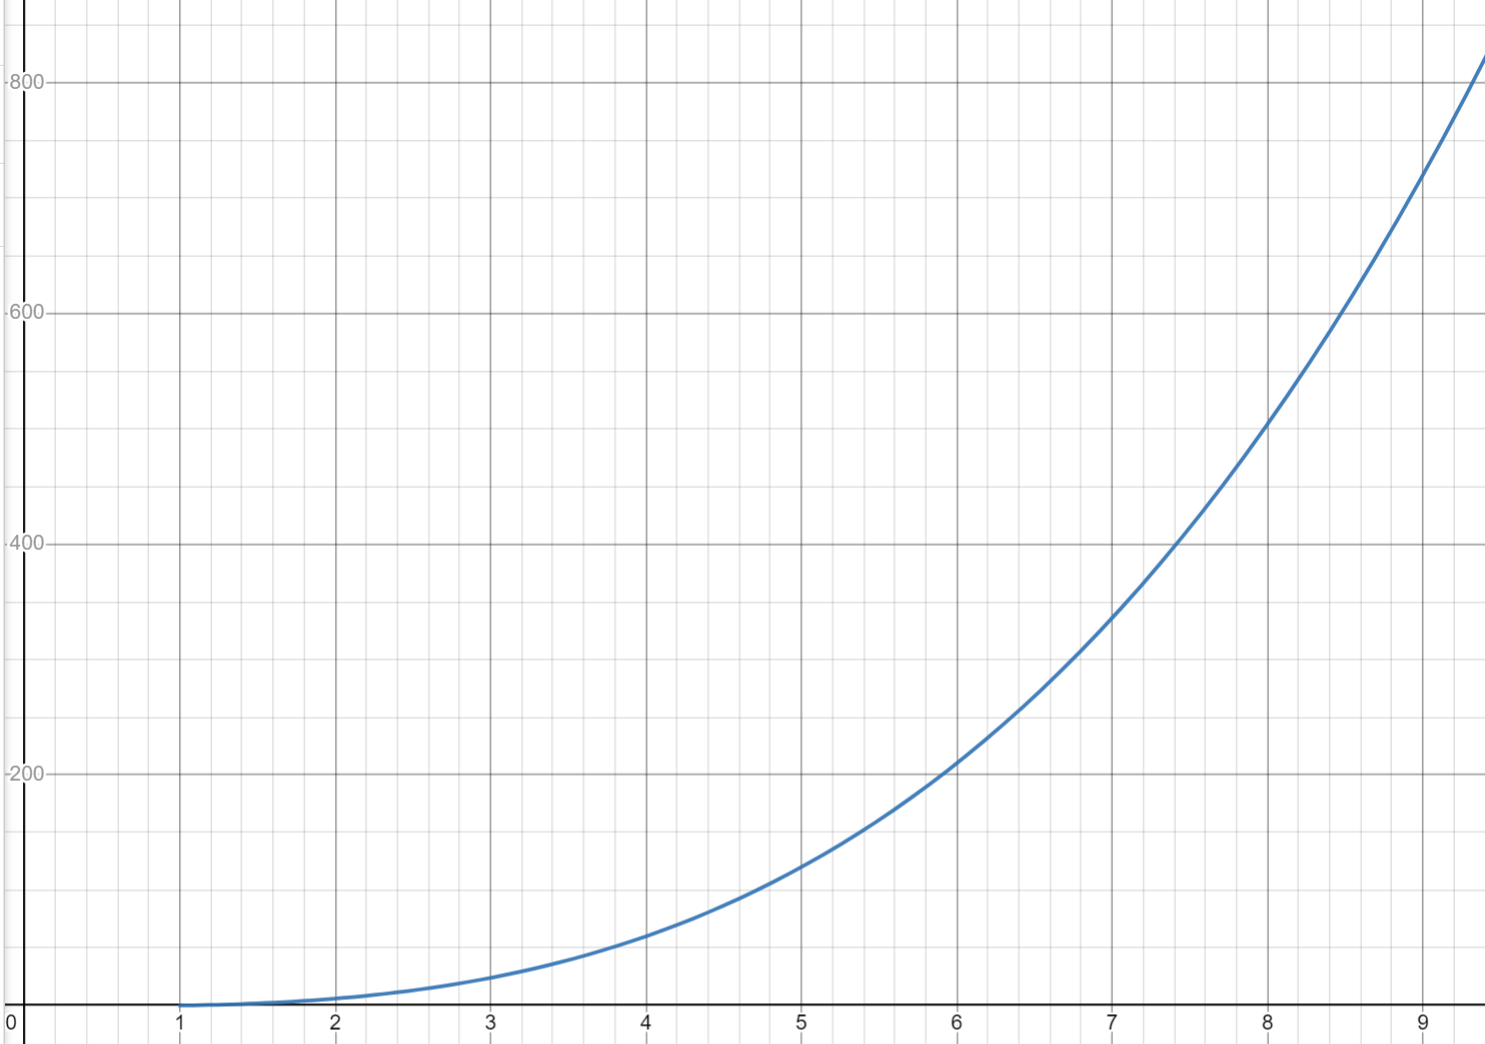
\includegraphics[scale=0.5]{Munkres6G.png}
    \\\\ Graph for $g^{-1}$:
    \newline 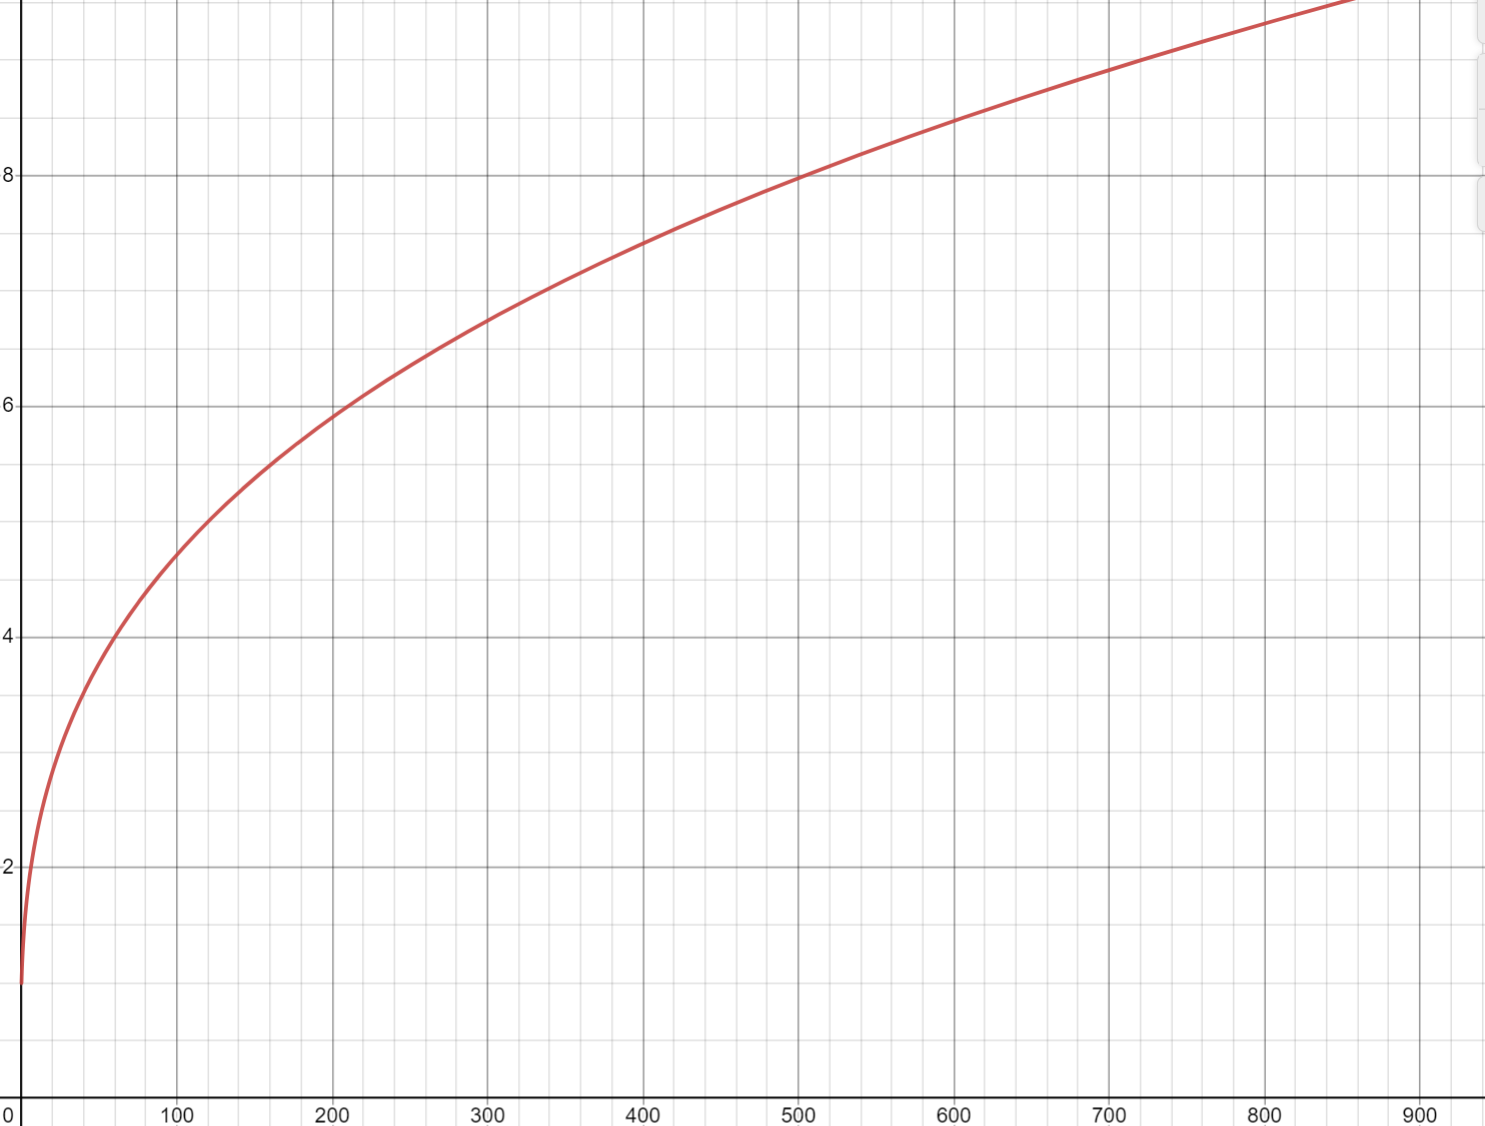
\includegraphics[scale=0.5]{Munkres6GInverse.png}
    
\end{enumerate}




\end{document}
